\chapter{Problem Statement}
\label{chap:problemStatement}
This chapter builds upon the related works presented in \cref{chap:relatedWork}, which represent the current state of the art for our problem, and the background concepts introduced in \cref{chap:background}, which describe decentralized technologies with a focus on the blockchain. It delves into the specific problem addressed by this work, and introduces the use case that guided the design of \gls{ew}.

As introduced in \cref{chap:introduction}, our problem is the management of secure and verifiable academic information. Since we are rapidly moving into Web3 technologies, students and institutions require a decentralized system of records-keeping that enables them to share these information without the use of traditional document and validation methods. Based on the related works discussed earlier, such a system must cover all aspects of a student's academic career and provide stakeholders with a streamlined environment that prioritizes \gls{ux} and interaction. More in detail, \gls{ew} aims to enable university to issue certificates and record courses evaluation in a tamper-proof and secure system, leveraging on blockchain characteristics to provide these features. 

On the students side, instead, we want to follow Web3 rule about data ownership and design a system in which students are the owner of their academic data; this means that they can manage the access to their academic wallet and decide the entity that can view and modify their information.

%%%%%%%%%%%%%%%%%%%%%%%%%%%%%%%%%%%%%%%%%%%%%%%%%%%%%%%%%%%%%%%%%%
% USE CASE
%%%%%%%%%%%%%%%%%%%%%%%%%%%%%%%%%%%%%%%%%%%%%%%%%%%%%%%%%%%%%%%%%%
\section{Use Case}
By analysing this problem, we developed a use case, illustrated in \cref{fig:sequenceDiagram}, to simulate the usage of \gls{ew}. The scenario involves four main actors:
\begin{itemize}
    \item The \textbf{home university}, which issues certificates and records evaluations during the student's regular academic career.
    \item The \textbf{host university}, which requires access to the student's academic data when the exchange project begins.
    \item The \textbf{student}, who participates in an exchange project, such as the Erasmus+ program. At the beginning of the program, they must send their academic history to the host university. At the end of the program, the home university must certify the results obtained at the host institution.
    \item The \textbf{administrator} of the \gls{ew} system, who manages the registration of students and universities in the platform.
\end{itemize}

\begin{figure}
  \centering
  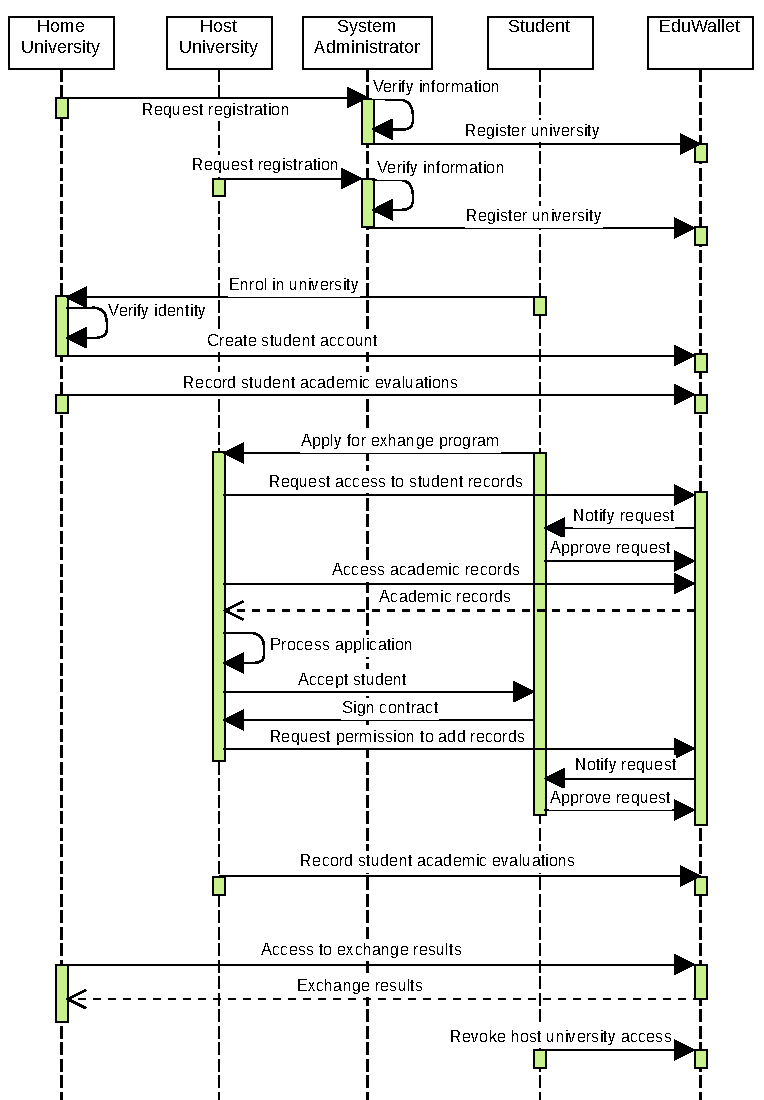
\includegraphics[width=0.7\textwidth]{figures/Sequence diagram.pdf}
  \caption[Sequence diagram of the EduWallet use case]{Sequence diagram illustrating the chronological interactions between student, universities, EduWallet, and the system administrator during the academic exchange process.}
  \label{fig:sequenceDiagram}
\end{figure}

The first step is the registration of universities in the \gls{ew} system. Universities request access from the system administrator, who verifies their information and, upon approval, registers them into the platform.

Once the universities are present in the system, the student begins their academic career by enrolling in the home university. As with traditional enrolment, the university verifies the student's identity and, once validated, creates an account for them in \gls{ew}. With the account created and the appropriate permissions, the home university can begin registering the student's academic evaluation.

After some years of regular study, the student decides to participate in an exchange program at the host university. To process the application, the host university needs access to the student's academic records. It sends a request via \gls{ew}, which the student receives and approves by granting the necessary permission.

Once granted access, the host university retrieves the student's history directly from \gls{ew} and proceeds with the application. Upon acceptance, the students signs the learning agreement and begins the program. The host university then requests permission to add new academic records to the student's wallet. The student again approves this request.
After completing the exams, the host university record the evaluations in the student's account. At the end of the exchange program, the home university accesses the list of completed courses from \gls{ew} to update the student's academic career.

Finally, the student revokes the host university access permissions, as they no longer need access to their academic wallet. The student and both universities have successfully completed the streamlined management of exchange program documentation using \gls{ew}. 

The scenario highlights the need for a system that balances security with usability, while ensuring that students retain control over their academic data. The key features required in such a solution include secure credential management, decentralized data ownership, streamlined inter-institutional communication, and tamper-proof record keeping. The following chapter translates the features outlined in the use case and problem analysis into specific requirements for the \gls{ew} system.